\section{讨论}\label{sec:discussion}

\subsection{两个子主张的回答汇总}\label{sec:disc-summary}

表 \ref{tab:summary} 把 S1 / S2 与本文全部证据对上。
一句话总结：\textbf{固定大小的持续状态确实承载了可测的跨上下文信息（S1 成立），
但它的有效记忆距离只有 $1$--$4$k token（S2 部分成立）}；
而这两件事的承载者都是块级循环状态，不是那个参数量最大的矩阵记忆。

% 7.1 汇总表：子主张 × 证据 × 图表 × 判定
\begin{table}[H]
\centering
\caption{S1 / S2 的判定汇总。每个判定句都由对应小节的末句直接给出，可逐条回查。}
\label{tab:summary}
\small
\begin{tabular}{@{}p{0.10\linewidth}p{0.30\linewidth}p{0.43\linewidth}p{0.10\linewidth}@{}}
\toprule
子主张 & 证据（实验） & 关键数字 & 判定 \\
\midrule
S1（有没有） &
A1 热启动 vs 空白 &
同窗口 $1.588$ vs $5.319\bits$（差 $+3.731$），窗口内无收敛趋势 &
\textbf{成立} \\
\addlinespace[2pt]
S1（有没有） &
A2 写入 vs $\mathit{lock}$ &
成对差 $+0.999\pm0.095\bits$；差值前段 $0.585\to$ 后段 $0.771\nats$ &
\textbf{成立} \\
\addlinespace[2pt]
S1（谁承载） &
A5 单组件重置 / A6 冻结 / B2-freeze &
冻结 \texttt{recurrent} $+1.022\bits$（$\approx$ 全锁 $+1.034$）；冻结 \texttt{memory} $-0.0005$；
边界冲击 $0.378/0.450\nats$ &
跨 patch 适应由 \texttt{recurrent} 承载 \\
\addlinespace[2pt]
S2（有多少） &
B1-lite + E5 重置频率 &
96/512\,KB 漂移无尖峰；重置周期 $512\to\infty$：$1.2147\to1.0385\bits$ 单调 &
长度非瓶颈 \\
\addlinespace[2pt]
S2（有多少） &
B2 距离分桶 + B2-freeze &
$<\!1$k 增益 $+0.0839\nats$（9384 对），$4$k 外 $\approx0$；冻结 \texttt{recurrent} 抹平增益 &
\textbf{有效记忆 $\approx1$--$4$k token} \\
\addlinespace[2pt]
S2（折算窗口） &
B3 等效滑窗基线 &
\pending{未完成} &
待定 \\
\addlinespace[2pt]
边界能力 &
B4 needle 预实验 / G1 合成绑定 &
合成键值对绑定弱（$8.3$--$8.6$ bits $\approx$ 机会线） & 限定 claim（\S\ref{sec:limits}） \\
\midrule
评测去污染 &
D2b 成员推断 &
状态级样本记忆 $-0.714\bits$；热启动 train gap $-0.350\pm0.200$，空白 $+0.365\pm0.828$ &
\textbf{主表须双报起点状态} \\
\bottomrule
\end{tabular}
\end{table}


\subsection{设计启示：状态接口的可操纵性}\label{sec:disc-design}

本文所有实验的旋钮都落在架构暴露的接口上，没有一处需要改权重、改数据或改提示词。
这一点的工程含义值得单独记下来：

\begin{itemize}\itemsep3pt
\item \textbf{$\mathit{lock}$ 天然给出受控对照}：因为首个 patch 的输出与正常前向逐位一致
（此时尚未发生写入），两组条件在第一步严格相同，差异只能来自后续的写入行为——
这比「同一模型跑两次但初始化不同」之类的对照干净得多。
\item \textbf{状态不可变 $\Rightarrow$ 实验可并行、可回滚}：每个 patch 后拿到的是新状态对象，
因此可以在同一条快照上同时开出「只重置 \texttt{memory}」「只清零 \texttt{recurrent}」
「冻结 \texttt{queue}$+$\texttt{MTM}」等多个分支而不互相污染。
\item \textbf{组件粒度可到下界}：把「跨 patch 写入」这一整块干预拆成四个分量版本后，
归因结论直接落在分量上（\S\ref{sec:s1-attr}）——
这在 RNN 的隐状态上看不到，因为隐状态没有暴露「按分量置换」的接口。
\end{itemize}

\textbf{代价与纪律}：状态跑一次就变，任何复用都会造成实验间污染；
因此每次评测必须先克隆，且快照必须落盘（本架构的状态一旦被改写无法复原）。

\subsection{与其他实验线的关系与展望}\label{sec:disc-rest}

\subsubsection{状态里装的是什么（D 线）}\label{sec:dline}

A1 说明热启动状态很值钱（$3.73\bits$），D 线回答它值钱在哪里（表 \ref{tab:d1}）。
四个文本档上的 gain（空白 $-$ 热启动）为：\textbf{同分布} $+5.061\pm0.580$、
\textbf{跨域}（sft 尾部）$+4.373\pm0.912$、\textbf{同分布但字节打乱} $-0.314\pm0.331$、
\textbf{零信息}（全空格）$+2.688$（图 \ref{fig:d1}）。
解读：热启动记忆的主体是\textbf{通用序列先验}（跨域仍保留 $\sim4.4\bits$），
叠加少量\textbf{同分布偏向}（$\sim0.7\bits$）；对打乱字节没有先验，
说明记忆锚定的是自然语言的\emph{结构}而不是字节取值本身。

% D1 / D2 / D2b：热启动记忆的性质
\begin{table}[t]
\centering
\caption{D 线：热启动状态里装的是什么（4\,KB $\times$ 5 seed，95\% CI）。
（a）D1 领域分解：gain $=$ 空白 $-$ 热启动，四档文本；
（b）D2/D2b 成员推断：训练消费区 vs 未消费同分布文本，以及「去掉热启动」后的同一比较。
热启动的收益主要是通用序列先验（跨域仍在），含少量同分布偏向；
而\textbf{逐样本的训练痕迹几乎全部由状态承载}（去掉热启动后 train gap 消失）。}
\label{tab:d1}
\small
\begin{tabular}{@{}lccc@{}}
\toprule
\multicolumn{4}{@{}l}{\textbf{(a) D1 四档文本（4\,KB $\times$ 5 seed）}} \\
\midrule
文本档 & 热启动 (bits/byte) & 空白 (bits/byte) & gain（空白 $-$ 热启动） \\
\midrule
同分布 held-out & $1.323\pm0.239$ & --- & $+5.061\pm0.580$ \\
跨域（sft 尾部） & $1.681\pm0.081$ & --- & $+4.373\pm0.912$ \\
同分布但字节打乱 & $11.901\pm0.463$ & --- & $-0.314\pm0.331$ \\
零信息（全空格） & $0.236$ & --- & $+2.688$ \\
\midrule
\multicolumn{4}{@{}l}{\textbf{(b) D2 / D2b 成员推断}} \\
\midrule
条件 & 消费区 (bits/byte) & 未消费 (bits/byte) & gap（消费 $-$ 未消费） \\
\midrule
热启动（权重 $+$ 状态） & $0.973\pm0.173$ & $1.323\pm0.239$ & $-0.350\pm0.200$ \\
空白（仅权重） & --- & --- & $+0.365\pm0.828$ \\
\midrule
\multicolumn{4}{@{}l}{状态级样本记忆 $=$ 热启动 gap $-$ 空白 gap $= \mathbf{-0.714}$ bits/byte} \\
\bottomrule
\end{tabular}
\end{table}


\begin{figure}[t]
\centering
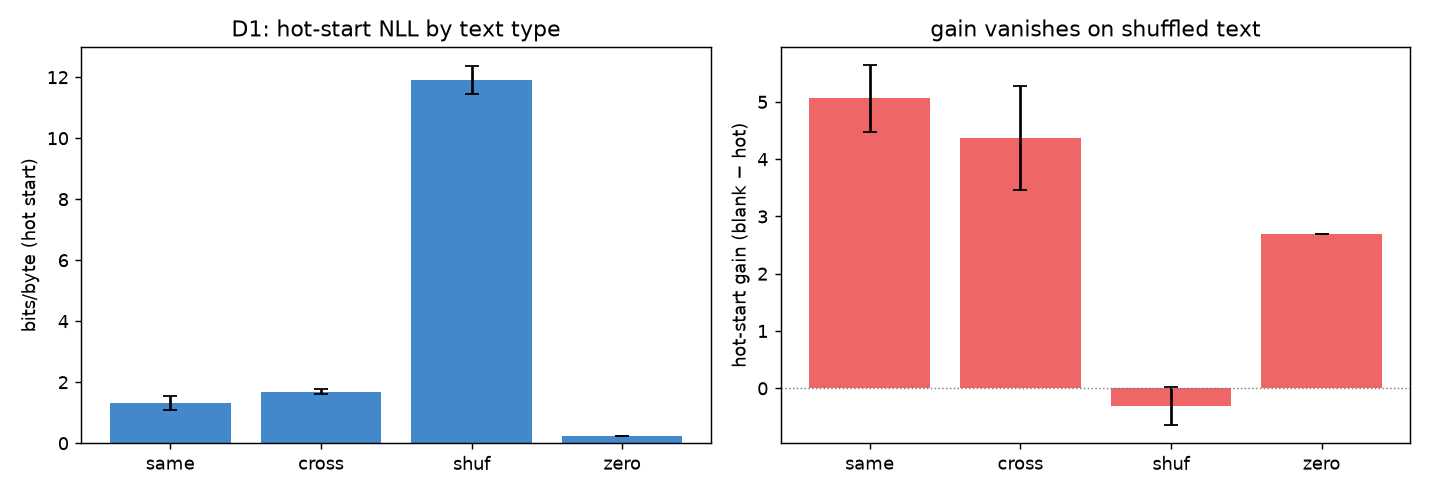
\includegraphics[width=\linewidth]{fig_d1_domain.png}
\caption{D1：热启动记忆的领域分解（4\,KB $\times$ 5 seed）。左：各档文本的热启动 NLL；
右：gain（空白 $-$ 热启动）——跨域仍保留大部分收益，打乱字节的收益为负。}
\label{fig:d1}
\end{figure}

\textbf{成员推断（D2 / D2b）是必须公开的一条。}训练消费区文本在热启动下的 NLL 比未消费同分布文本低
$-0.350\pm0.200\bits$；把起点换成空白后这个差距消失（$+0.365\pm0.828$，与 0 无显著差异），
反推\textbf{状态级样本记忆} $=-0.714\bits$。也就是说：\emph{逐样本的训练痕迹几乎完全由状态承载，权重没有贡献}。
两个含义：其一，评测协议上任何用热启动的数字都带着「这几段文本模型可能见过」的脚注，
主表必须双报起点状态（\S\ref{sec:cond}）；其二，隐私与去污染上，状态本身是记忆载体，
这不只是统计压缩问题。

\subsubsection{超长上下文的数值安全（E 线）}\label{sec:eline}

96\,KB 单流：$\|\texttt{memory}\|_F\times1.018$、$\|\texttt{MTM}\|_F\times1.019$，
\texttt{recurrent}/\texttt{queue} 范数构造性恒定；
512\,KB 单流：$\times1.132$ 与 $\times1.065$（图 \ref{fig:e1} 左、图 \ref{fig:e1long} 左）。
全程有界缓增、未见发散——这是 delta 规则 $+$ $1/\mathrm{eff\_seq\_len}$ 门控在数值上的正面证据。

\textbf{污染与自愈（E2）}：正常 8\,KB $+$ 随机字节 4\,KB $+$ 正常 8\,KB 的流上，
污染段内的 NLL 冲击为 $+9.25$（照常写入）与 $+9.92\nats$（污染段设为只读）；
但\textbf{两组条件的尾部 NLL 只差 $0.0001$}（$0.8608$ vs $0.8607$），残留都是 $+0.085\nats$。
结论有两层：污染写入只造成\textbf{瞬时冲击}（污染后头 4 个 patch：$0.686$ vs $0.436\nats$），
\textbf{没有长期残留}；也因此「只读模式可作污染防御」这一说法\textbf{得不到数据支持}——
残留量在两个条件下相同，尾部抬升更可能来自文本难度变化（与 \S\ref{sec:b1} 的漂移解释一致）。
图见附录 \ref{app:eline}。

\subsubsection{前向学习：连续适应而非离散绑定（G 线）}\label{sec:gline}

持续状态的另一面是「读着读着就变了」。合成任务上的结果（附录表 \ref{tab:g}、图 \ref{fig:g1}、\ref{fig:g1c}）
可以概括为一句话：\textbf{这个检查点上的前向学习是连续适应，而不是离散绑定}。
（i）随机 ASCII 键值对联想：$k$ 次演示后 write 条件仍在 $8.3$--$8.6$ bits
（机会线 $8.23$），且不随 $k$ 累积；write 与 $\mathit{lock}$ 的差只有 $+0.37$--$+0.66\bits$。
（ii）把符号换成分布内高频词对后曲线\textbf{完全变平}（$5.0$--$5.2$ bits，与首字节机会线重合），
说明这\textbf{不是}合成数据 OOD 造成的——是 delta 规则通道对离散配对的绑定本身很弱。
（iii）自然语料上的 $8$-gram 复现增益只有 $+0.054\nats$，且在 $\mathit{lock}$ 下消失。
把这三条与 A2/A6 的 $+1.00\bits$ 放在一起看，\textbf{跨 patch 的收益主要来自连续的话题/句法适应，
而不是「记住若干条事实」}。这既是本文的机制结论，也是把 needle 类精确检索降级为限定 claim 的直接理由（\S\ref{sec:b4}）。

\subsubsection{下一步：训练侧实验（F 线）}\label{sec:f-line}

本文的全部证据都指向同一个未解问题：为什么有效记忆只有 $1$--$4$k token？
是\textbf{机制上界}（固定状态在这个写入规则下就只能记这么久），
还是\textbf{训练进度}（该检查点只训到 20\%，长程写入尚未学出来）？
这需要训练侧实验才能分辨，按优先级：

\begin{enumerate}\itemsep3pt
\item \textbf{BPTT 窗口扫描}（$\mathrm{bptt}=1/4/8$）：$\mathrm{bptt}=1$ 时梯度只到 patch 内，
长程信用\textbf{只能}经前向 delta 规则传递。它的长程表现保留多少，
即「前向通道」的贡献上限；$1\to4$ 的增益即梯度通道的贡献。
这是本文「持续学习」主张在训练侧的判决性实验。
\item \textbf{永续 vs 文档边界重置训练}：直接检验「训练时不清状态到底是收益还是负担」。
\item \textbf{状态收敛（F5）}：用早期/中期/晚期检查点比较热启动收益与状态间相似度，
回答「热启动之所以有效」的前提是否稳定。
\item \textbf{chunk\_size（并行流数）扫描}：v\_0d3 中 \texttt{memory} 的写入是跨流平均的，
流数直接改变「每流写入占比」；v\_0d4 改为序列级私有槽位后，流数变为「独立记忆实例数」，
该扫描在两版语义下问的是不同的问题——与推理 batch$=1$ 的匹配度直接相关。
\end{enumerate}

在这些实验完成之前，本文的结论应当被理解为\textbf{该检查点在该规模上的实测上界}，
而不是该架构的能力上界。
